The CEBAF accelerator at Jefferson Lab generates the electron beam used in the HPS experiment. CEBAF can deliver continuous electron beams to multiple experimental halls simultaneously. The CEBAF accelerator is a recirculating linac in the shape of a racetrack through which electron beam bunches can pass multiple times, boosted in energy with each pass, before being delivered to a specific hall. 

\begin{figure}[htb]
  \centering
      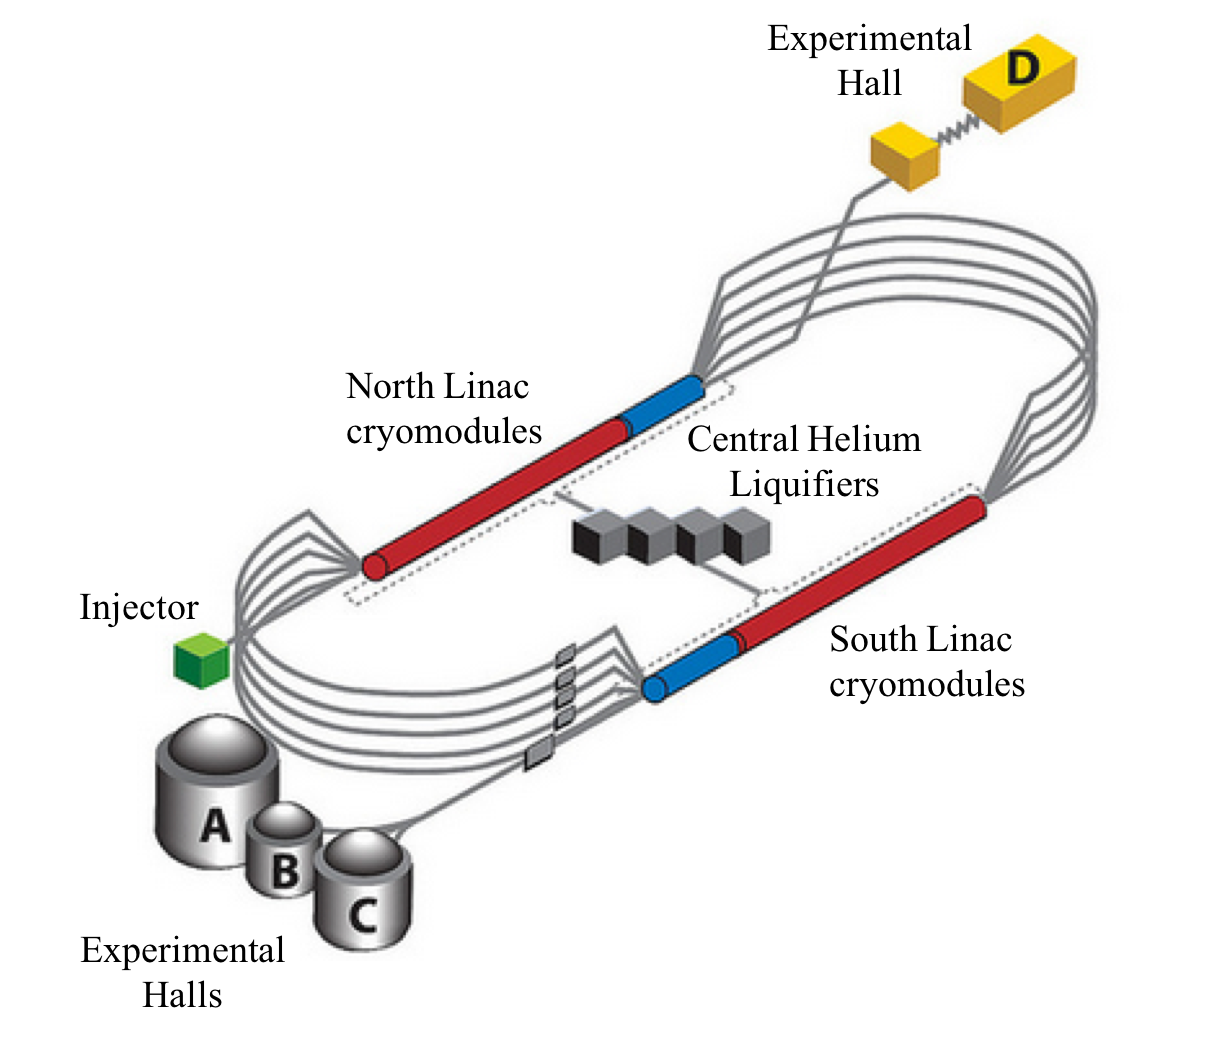
\includegraphics[width=0.75\textwidth]{pics/experiment/cebafLabel.png}
  \caption[CEBAF accelerator]{A drawing of the CEBAF accelerator is shown. The electron beam is produced at the injector and can circulate through up to five passes around the race track design of the accelerator. There are four experimental halls that can receive beam and run experiments, simultaneously: A, B, C, and D. CEBAF was upgraded prior to the HPS experiment to include additional cryomodules, a second Central Helium Liquifier (CHL), and a fifth pass in order to produce higher energy.}
  \label{Figure:cebaf}
\end{figure}

CEBAF can provide continuous electron beams with energies up to 12~GeV and intensities up to approximately 100~$\mu$A to each of the four experimental halls. CEBAF was upgraded from producing 1.1~GeV per pass to 2.2~GeV per pass in 2014. 
%The injector energy is 100~MeV, designed for a maximum of five passes (upgraded from four passes) with %an energy per pass of 2.2~GeV (upgraded from 1.1~GeV). These upgrades double the maximum energy %output of the accelerator. While the accelerator frequency operates at 1500~MHz, a new 750~MHz RF %separator was installed in order to provide beam to all four halls simultaneously. With these upgrades, the %halls can receive the beam at 250 or 500~MHz and operate at different energies \cite{Kazimi_2013}. 

HPS was the first experiment to run in Hall B after the accelerator was upgraded. After a problem occurred in one CHL during the Engineering Run in the spring of 2015, HPS obtained dedicated beam time as one of the few experiments that could continue to take physics data with the accelerator operating at a single pass using the remaining CHL. The resulting energy for the Engineering Run, 1.05~GeV, would have been impossible to obtain with the simultaneous running of other experiments requiring 2.2~GeV per pass.  
